\documentclass[doublespacing,12pt]{report}
\usepackage{graphicx}
\usepackage{tocbibind}
\usepackage{hyperref}
\usepackage{amsmath}
\usepackage{graphicx}
\usepackage{array}
\usepackage{booktabs}
\usepackage{geometry}
\geometry{a4paper,margin=1in}
\usepackage{float}
\usepackage{amsfonts}
\usepackage{lmodern}
\usepackage{setspace}
\usepackage{enumitem} 
\usepackage{tabularx} % Add this line in the preamble
\usepackage{geometry}
\usepackage{titlesec} % Add this package

% Customizing chapter titles
\titleformat{\chapter}[display]
  {\normalfont\Huge\bfseries\centering} % Increased font size to \Huge and centered
  {\chaptername\ \thechapter}{20pt}{\Huge} % Adjust the second \Huge to control title text size

% Reduce the margin at the top of each chapter
\titlespacing*{\chapter}{0pt}{-40pt}{20pt} % Adjust the -20pt to reduce the space above

\begin{document}

\pagenumbering{gobble} % No page numbers 
\begin{singlespace} % Start single spacing
\begin{titlepage}
\centering
   % \vspace{0.2cm}
    \large\textbf{KWAME NKRUMAH UNIVERSITY OF SCIENCE AND TECHNOLOGY}

    %\Huge\textbf{(KNUST)}
    %\vspace{0.2cm}
      \vspace{0.2cm}
  \large\textbf{DEPARTMENT OF STATISTICS AND ACTUARIAL SCIENCE}
    %\vspace{0.2cm}
    
     \begin{center}

\includegraphics[width=0.6\textwidth]{logo.png}\end{center}

   \large{\textbf{\MakeUppercase{Decoding Student Retention and Churn of Vodafone (Telecel) in Kwame Nkrumah University of Science and Technology (KNUST): A Survival Analysis Approach}}}
\vspace{0.4cm}
   \\
   %\large{\textbf{A Survival Analysis Approach}}
    \vspace{0.4cm}
    
\large{Musah Faridu Oubda\\
Kassim Asana\\
Sarpong Linda\\
Torsi Edmond Collins\\
Asiamah Ezekiel}

    \vspace{0.4cm}  
    \small{A THESIS SUBMITTED TO THE DEPARTMENT OF STATISTICS AND ACTUARIAL SCIENCE, KWAME NKRUMAH UNIVERSITY OF SCIENCE AND TECHNOLOGY IN FULFILLMENT OF THE REQUIREMENT FOR THE AWARD OF THE DEGREE OF BACHELOR OF SCIENCE IN ACTUARIAL SCIENCE}\\
    \vspace{0.4cm}
    {AUGUST , 2024}
\end{titlepage}
\end{singlespace} % End single spacing


% Start numbering with Roman numerals for the Declaration
\pagenumbering{roman}

\chapter*{Declaration}
\addcontentsline{toc}{chapter}{Declaration}



We, therefore, affirm that this paper is entirely our own original work and has not been submitted in whole or in part for another degree award in any other university. Due credit has also been given to previously published works and online publications through referencing. 
\vspace{0.1in}

\newpage
\begin{tabbing}
    \hspace{6cm} \= \hspace{4cm} \= \hspace{5cm} \kill
    \textbf{Musah Faridu Oubda} \> \makebox[4cm]{\dotfill} \> \makebox[4cm]{\dotfill} \\
    {Index No. (4325620)} \> {Signature} \> {Date} \\[1.5cm]
    \textbf{Kassim Asana} \> \makebox[3cm]{\dotfill} \> \makebox[3cm]{\dotfill} \\
    {Index No. (4323020)} \> {Signature} \> {Date} \\[1.5cm]
    \textbf{Sarpong Linda} \> \makebox[3cm]{\dotfill} \> \makebox[3cm]{\dotfill} \\
    {Index No. (4330720)} \> {Signature} \> {Date} \\[1.5cm]
    \textbf{Torsi Edmond Collins} \> \makebox[3cm]{\dotfill} \> \makebox[3cm]{\dotfill} \\
    {Index No. (4331420)} \> {Signature} \> {Date} \\[1.5cm]
    \textbf{Asiamah Ezekiel} \> \makebox[3cm]{\dotfill} \> \makebox[3cm]{\dotfill} \\
    {Index No. (4316720)} \> {Signature} \> {Date} \\[1.5cm]
\end{tabbing}

\begin{tabbing}
    \hspace{6cm} \= \hspace{4cm} \= \hspace{5cm} \kill
    \textbf{Certified by:}\\ 
    \textbf{Miss Sandra Addai-Henne} \> \makebox[3cm]{\dotfill} \> \makebox[3cm]{\dotfill} \\
    {Supervisor} \> {Signature} \> {Date} \\[1.5cm]
    \textbf{Certified by:}\\ 
    \textbf{Prof. Gabriel Asare Okyere} \> \makebox[3cm]{\dotfill} \> \makebox[3cm]{\dotfill} \\
    {Head of Department} \> {Signature} \> {Date}
\end{tabbing}



\newpage
\chapter*{Abstract}
\addcontentsline{toc}{chapter}{Abstract}

This study examines the factors influencing student churn at Kwame Nkrumah University of Science and Technology (KNUST), with a particular focus on the telecommunications services provided by Vodafone (now Telecel). Utilizing survival analysis methods, including the Cox Proportional Hazards (PH) model and the Lognormal Accelerated Failure Time (AFT) model, the research identifies key predictors of churn and analyzes survival rates across different academic levels. The findings indicate that poor network quality significantly increases both the churn rate and the time to churn. While the Cox PH model demonstrates superior predictive value, the Lognormal AFT model offers a better overall fit. The result has important implications for both Telecel and KNUST, suggesting that enhancements in network quality could improve student retention. The study concludes with recommendations for reducing churn and outlines directions for future research.


\newpage
\chapter*{Acknowledgment}
\addcontentsline{toc}{chapter}{Acknowledgement}

We are grateful to the Great and Mighty God for giving us the ability and fortitude to do this task. Our sincere gratitude also extends to Miss Sandra Addai-Henne, our supervisor, who acted as a beacon of hope for us as we set out on our path. We will always remember her kindness, comprehension and level of tolerance. She always mentored and corrected us. We also want to express our gratitude to all of the instructors at Kwame Nkrumah University of Science and Technology(KNUST) who assisted us with our studies. We are grateful to you everyone.  



\newpage
\chapter*{Dedication}
\addcontentsline{toc}{chapter}{Dedication}


We dedicate this project to the Almighty God, who has seen us through all of our challenges during this thesis period and has brought us this far. We also dedicate this effort to our families and friends, who have been there for us every step of the way with love and prayers. Finally, we dedicate this presentation to our supervisor, who stood by us through it all.  

\newpage
\chapter*{List of Abbreviations}
\addcontentsline{toc}{chapter}{List of Abbreviations}

\begin{tabbing}
    \textbf{ACE} \hspace{2cm} \= Africa Coast to Europe \\
    \textbf{AFT} \> Accelerated Failure Time \\
    \textbf{AIC} \> Akaike Information Criterion \\
    \textbf{AT} \> AirtelTigo \\
    \textbf{BIC} \> Bayesian Information Criterion \\
    \textbf{CDF} \> Cumulative Distribution Function \\
    \textbf{CPHM} \> Cox Proportional Hazard Model \\
    \textbf{CPH} \> Cox Proportional Hazard \\
    \textbf{C-index} \> Concordance Index \\
    \textbf{GSES} \> Ghana Satellite Earth Station \\
    \textbf{HQ} \> Hannan-Quinn Criterion \\
    \textbf{KM} \> Kaplan-Meier \\
    \textbf{KNUST} \> Kwame Nkrumah University of Science and Technology \\
    \textbf{PDF} \> Probability Density Function \\
    \textbf{PH} \> Proportional Hazards \\
    \textbf{RSF} \> Random Survival Forest \\
    \textbf{SA} \> Survival Analysis \\
    \textbf{S(t)} \> Survival Function \\
    \textbf{SMS} \> Short Message Service \\
    \textbf{UITS} \> University Information Technology Services \\
    \textbf{WACS} \> West Africa Cable System \\
    \textbf{h(t)} \> Hazard Function \\
\end{tabbing}



\newpage
\renewcommand{\contentsname}{Table of Content} % Rename the Table of Contents
\tableofcontents % Generate the Table of Contents


\newpage
\listoffigures

\newpage
\listoftables



 




\newpage
\chapter{Introduction}

% Start numbering from here
\pagenumbering{arabic}

\section{Background of Study}

Ghana's telecommunications industry has experienced significant growth in recent years, with companies such as Vodafone playing a crucial role in providing mobile and internet services to people across the country [Bandim, 2022]. The industry is highly competitive, making customer retention vital for sustaining market share and profitability. Obtaining new customers is more expensive than retaining existing ones due to marketing activities, incentives and campaigns involved. Therefore, retaining a customer is preferable to acquiring a new one. Customer churn, also known as customer attrition, refers to the loss of subscribers or customers who cease using a company’s service or product within a given period [Koranchirath, 2024]. Understanding the reasons behind customer churn helps to develop strategies to improve customer retention and help reduce churn rates in the long run.\\
Vodafone is one of the leading national telecommunications providers in Ghana. As of January 2020, it had over 9.3 million mobile voice subscribers, representing 13.81\% of Ghana's market share. Since becoming the majority shareholder, Vodafone Ghana has been operating the Ghana Satellite Earth Station (GSES) since 2008 [Wikipedia, 2020]. GSES allows Ghana to access and utilize communications satellites orbiting the Earth for various applications, such as telephone services, internet connectivity, television broadcasting, data transmission, disaster management and emergency communications. The operation of the earth station by Vodafone Ghana proves the company's commitment to investing in and upgrading Ghana's satellite communications capabilities.\\
In 2016, Vodafone partnered with Kwame Nkrumah University of Science and Technology (KNUST) to provide enhanced packages of services to the various faculties across the university's campuses to improve education services [Wikipedia, 2020]. This collaboration included telecommunications services such as SIM cards and data plans for the student and employee communities.\\
In February 2023, Telecel acquired 70\% shares in Vodafone, rebranding the company name to Telecel in 2024 [Wikipedia, 2024]. This rebranding aimed to improve service offerings across voice and data services, money transfers and business solutions. Telecel, founded in 1986, is an Africa-focused telecommunication company that operates primarily in Africa and converges telecommunications with fintech, e-commerce and tech startups.\\
Student churn is a major issue every telecom company encounters. It leads to a loss of revenue and increases the cost of acquiring new customers. In the highly competitive telecom market, where customers have multiple service provider options, retaining customers becomes even more challenging. Companies use modern technology, computer software and survival analysis approaches to identify at-risk students and devise strategies to enhance retention rates. This method of recognizing unsatisfied customers is known as churn prediction.\\
On March 14, 2024, Vodafone, along with several other telecommunications companies, was hit by outages on several underwater fiber optic cables, leading to disruptions in services, particularly internet services [Ghana Web, 2024]. It affected about 10 countries in West Africa, including Ghana. Initially, it was estimated that the problem would be fixed within 3 days; however, this was not the case. The damage was massive, affecting the West Coast route to Europe, West Africa Cable System (WACS) and the Africa Coast to Europe (ACE), resulting in MainOne and SAT3 going offline [AP News, 2024]. The only network that was properly functioning at the moment in Ghana was AirtelTigo (AT). To quickly prevent the loss of valuable customers to AirtelTigo, Vodafone (Telecel) took the initiative to update its customers daily on their progress and offer various bonuses to prevent customers from defecting to their competitors. This continued until the problem was fixed on April 29, 2024, when the WACS cable was repaired.\\
Previous studies have explored various factors that influence customer churn in a telecommunications company. This study aims to focus on the KNUST student population, uncover and analyze data gathered from students, apply survival analysis models to identify patterns related to churn (such as demographics, usage patterns, etc.), develop retention strategies, evaluate the success of these efforts and make informed decisions.

\section{Problem Statement}

Despite KNUST's efforts to partner with Telecel for affordable and accessible mobile communication services, student churn remains a persistent issue. The core problem lies in the insufficient understanding of the factors influencing student churn and retention, which hampers the development of effective strategies to tackle the issue [Kapur, 2018]. This research aims to address this gap by investigating the factors contributing to student churn and developing a survival analysis model to identify students at risk. The goal is to create targeted strategies that improve retention rates based on the model's insights.\\
The existing gap in knowledge regarding the precise reasons behind student churn undermines the ability to devise targeted interventions that could effectively address the issue. As a result, the strategies that have been implemented so far have not achieved the desired outcomes in reducing churn rates. This research seeks to bridge this gap by thoroughly investigating the various factors contributing to student churn and by developing a robust survival analysis model to accurately identify students who are at risk of churning. The objective is to leverage the insights gained from this model to design and implement targeted strategies aimed at improving retention rates. By addressing these issues, the research aims to facilitate understanding of churn dynamics and ultimately enhance the effectiveness of retention efforts.

\section{Research Objectives}
The objectives of the research is ;
\begin{enumerate}
\item To use survival analysis to estimate student churn rates at various academic years.
\item To determine which covariates affect the churn rate.
\item To provide strategies to combat churn.
\end{enumerate}
%\subsection{Main Objective}
%\begin{itemize}
    %\item 
%	To develop a survival analysis techniques model to detect at-risk students to improve student retention and reduce churn of Telecel at KNUST.
%	%\end{itemize}
%	
%	\subsection{Specific Objectives}
%	\begin{itemize}
%	    \item Exploring the factors that influence student churn and retention.
%	    \item Using survival analysis models to identify students at risk of churning.
%	    \item Analyzing time-to-event data to understand the patterns and timing of student churn.
%	    \item Identifying strategies to improve retention rates and reduce churn.
%	\end{itemize}

%\section{Research Questions}
%\begin{itemize}
%    \item What factors influence student retention and churn for Telecel services at KNUST?
%    \item What is the relationship between student demographics (age, gender, year of study) and churn behavior?
%    \item How does the churn rate vary with different Telecel services (voice service, data service, internet service)?
%    \item How does the quality of Telecel network and services (coverage, internet speed) influence student retention and churn?
%    \item How can Telecel services be optimized to better meet the needs and preferences of KNUST students?
%\end{itemize}

\section{Significance of the Study}

The study offers a comprehensive understanding of the factors impacting student churn from Vodafone. This will enable the development of precise strategies to enhance retention rates, thereby minimizing churn. The study will empower KNUST to improve the telecom services offered to its students. By identifying the factors influencing student retention and churn, KNUST can work closely with Telecel to guarantee the delivery of top-notch, dependable services to its students, thereby solidifying the partnership between KNUST and Telecel. The study is all about understanding what the populace expects from Vodafone (Telecel). By knowing their specific needs and preferences, the services can be improved upon. This means improved connectivity, service plans and less hassle from switching providers. Ultimately, it ensures a more stable and reliable service for students.

\section{Organization of the Study}

The study on student retention and churn for Telecel services at KNUST aims to investigate the factors that drive students' decisions on Telecel services usage. The study follows a structured approach. Chapter one discusses the background information and the foundation for the research. The problem statement and goals are stated here. Chapter two of the study contains a literature review, including several studies related to the subject at hand. The third chapter focuses on the methodology and data collection techniques. There are several ways of approaching this problem, but the main focus of the study is using a survival analysis modeling tool. The fourth chapter presents the models and practical application to the dataset. Detailed analysis is presented here with the aid of figures and diagrams to determine the optimal model for the research. Chapter five delves into the conclusion and summarizes the results obtained. Based on the findings, recommendations are formulated.

\section{Limitation of the Study}

The research is specifically concentrated on students within the College of Science at KNUST. As a result, it does not encompass students from other colleges within the university. This limitation means that the findings and insights derived from this study are relevant primarily to the College of Science and may not be fully applicable to students in other colleges.

\newpage
\chapter{Literature Review}


\section{Introduction}
Mobile technology has become widely used, changing how students interact, communicate and obtain information [Kapur, 2018]. Student retention and churn are critical issues for universities and telecom companies alike. In the context of Vodafone's services offered to students, understanding student behavior and preferences is crucial for effective retention strategies. This project addresses this gap using survival analysis, a statistical method for examining data over time [Box-Steffensmeier and Jone, 2020]. In this context, the event of interest is student churn, defined as the discontinuation or cessation of Vodafone SIM cards. By applying survival analysis, this project will provide valuable insights into student retention and churn factors.

\subsection{Telecommunication Industry and Customer Behavior}
The telecommunication industry is highly competitive, with customer acquisition and retention being pivotal to a company's success. Research indicates that factors such as service, pricing, customer support and competitive offerings significantly influence customer churn [Lai, 2021].

\subsection{Student Retention and Telecom Services}
Students, as a demographic, exhibit unique usage patterns and service expectations. Studies show that reliable connectivity, affordable pricing and additional benefits like educational resources influence their choice of telecom services [Smith and Brown, 2020]. For telecom companies, understanding these factors is crucial to tailoring services that meet students’ needs and enhance retention.

\subsection{History of Survival Analysis (SA)}
The origins of SA and its history spread far back to the early work on mortality by John Graunt, who published the book "Natural and Political Observations on the Bills of Mortality" in 1977. The concept of “Life Tables” was introduced in this book [Graunt, 1977]. A new, modern era in SA started during World War II in the USA, where the reliability of military equipment was tested using SA. After World War II, SA became popular and spread to various other disciplines [Jerenz, 2008]. The most influential papers on SA were published by Kaplan and Meier [Kaplan and Meier, 1958] and Cox [Cox et al., 1972], in which the Kaplan-Meier product limit estimator and Cox proportional hazard model were introduced, respectively.

\subsection{Application of Survival Analysis}
Survival analysis (SA) has been successfully applied in diverse fields, including medical research, engineering (reliability analysis), finance and economics. In finance, SA has been used to analyze a firm's vulnerability to global financial crises and identify firms at risk of failure, enabling timely interventions [Lee, 2014, Pereira, 2014, Kumar and Gepp, 2015, Iwasaki, 2014]. SA has also been employed to predict the optimal time to buy or sell stocks within the stock market [Kumar and Gepp, 2015]. In the banking sector, SA is utilized to assess banks' survival during financial crises, measure their strength when entering new markets [Leung et al., 2010, Evrensel, 2008] and conduct credit risk analysis [Tsujitani and Baesens, 2012, Baesens et al., 2005]. The widespread adoption of SA across these domains underscores its versatility and effectiveness in modeling time-to-event data and identifying the factors that influence outcomes of interest.

\section{Conceptual Review}

Customer retention refers to a company's capacity or ability to maintain or retain their customer base over a specific period. High retention rates are crucial for maintaining revenue streams, reducing marketing costs associated with acquiring new customers and fostering a positive brand reputation. Customer churn, also known as customer attrition, is the rate at which customers stop using a company's product or service [Masarifoglu and Buyuklu, 2019]. It can be caused by various factors such as dissatisfaction with the service, better offers from competitors, or changes in personal circumstances. In the telecommunications industry, market competitiveness is measured by churn rate. Telephone, internet and mobile services are all part of telecommunications.

\section{Empirical Studies}
%Include reference in the bibliography
A paper by [Imani, 2020] tackles customer churn in telecoms, emphasizing that retaining customers is cheaper than acquiring new ones. It evaluates various machine learning methods for predicting churn by comparing classifiers, target detectors, feature extraction and feature selection techniques. The study finds that Random Forest and Feed-Forward Neural Networks with Genetic Algorithm showed high accuracy. Effective target detectors included a Spectral wrangle Mapper and an Adaptive Subspace Detector. Clustering-Based Feature Extraction and Advanced Binary Ant Colony Optimization excelled in improving classification and feature selection. The study recommends implementing Random Forest and Neural Networks for effective churn prediction.\\
Another paper by [Masarifoglu and Buyuklu, 2019] emphasizes the importance of customer retention in telecoms, noting that retaining customers is more cost-effective than acquiring new ones. It employs survival analysis to estimate customer survival and hazard functions, focusing on factors like campaigns, tariffs, tenure, age and auto-payment. The paper introduces survival analysis (SA) as a statistical method to analyze time-to-event data. It describes the Cox Proportional Hazard Model (CPHM), a widely used technique for quantifying the risk of an event occurring during the observation period. The paper uses Kaplan-Meier estimates and the Cox model to analyze the impact of various predictors on customer churn. The results show how different factors, such as campaigns and tariffs, affect customer survival probabilities. The study finds that survival analysis is effective for predicting churn and recommends its use for targeting at-risk customers and improving retention strategies.\\
The CPH model, a well-established method, is known for its interpretability, allowing researchers to understand the relationship between covariates and survival time [Nurhaliza et al., 2022]. However, it assumes proportional hazards, which may not hold in all cases. In contrast, Random Survival Forest (RSF) is a non-parametric ensemble method that can handle complex, non-linear relationships and does not require the proportional hazards assumption. The study uses data from various domains, such as medicine and engineering, to assess the performance of both models. The findings suggest that while RSF generally offers better predictive accuracy, especially in cases with non-linear relationships, CPH remains valuable for its simplicity and interpretability. The paper concludes that the choice between CPH and RSF should be based on the specific requirements of the analysis, balancing the need for interpretability against predictive accuracy.




\newpage
\chapter{Methodology}

\section{Introduction}

This chapter structures the research methods and procedures followed by the analysis to predict student churn of Vodafone (Telecel) in KNUST. A comprehensive explanation of the research models, mathematical formulations and interpretations are presented here. The paper compares their performance using the Concordance Index thus shedding light on their predictive capabilities.

\section{Research Design}

The study employs quantitative research. This type of research aims to establish the cause-and-effect relationships between variables. Specifically, it focuses on quantifying various aspects of students’ usage and satisfaction, rather than exploring underlying meanings or personal experiences in an open-ended manner.

\section{Pilot Survey}

Before the actual study was carried out, a pilot survey was held to grasp the scope of students’ understanding of the topic. It was carried out using final year students in Actuarial Science. Out of 50 questionnaires sent out, a total of 46 answered the questions.
\section{Data Collection}

The primary data source for this research was a survey conducted among students at Kwame Nkrumah University of Science and Technology (KNUST) in College of Science. The survey targeted students in final years (Level 400). The dataset includes a variety of questions, each capturing specific aspects relevant to the study with the aid of Google Forms.


\section{Sample Size}
The sample size of the research was determined through simple random sampling. Simple random sampling is a sampling technique in which each member of the population has an equal chance of being selected. This method ensures that the sample is representative of the population, as every individual has an equal probability of being included. This sampling technique is employed to determine the optimal sample size as it is a straightforward method that allows for unbiased estimation of the population parameters.\\
The sample size for simple random sampling can be determined using the formula below:

\begin{equation}
n_0=\frac{z^2 \ast p \ast \left(1-p\right)}{E^2}
\end{equation}
\begin{equation}
n=\frac{n_0}{1+(\frac{n_0-1}{N})}
\end{equation}\\
Where:\\
\\
  \((N)\) is the population size.\\
  \((n_0)\) is the initial sample size for simple random sampling.\\
   \((n)\) is the adjusted sample size for the population.\\
  \((z)\) represents the critical value.\\
  \((p)\) is the estimated proportion of the population\\
 \((E)\) is the margin of error.\\

 

\section{Data Pre-Processing}

In the realm of data analysis, ensuring the quality and suitability of data is paramount for deriving meaningful insights and making informed decisions. The initial phase of the study involved a thorough examination of the dataset to identify and handle missing data appropriately to ensure that subsequent analyses were conducted on a complete and representative dataset. One of the critical preprocessing tasks involved the transformation of categorical variables into numeric format. This was achieved using label encoding, a technique that assigns unique integer labels to each category with the aid of Python. The transformation restructured the dataset to facilitate survival analysis. The data was then organized to facilitate essential components such as time duration, event indicators and relevant covariates to the variables. 
The lifelines package played a pivotal role in this section by providing essential survival analysis models in Python. The models are crucial for analyzing data where the time to student churn is important. 

\section{Concept of Survival Analysis}

Survival analysis is a branch of statistics used to analyze time-to-event data. The primary interest lies in the time until the occurrence of the event of interest.  The time variable is usually referred to as survival time since it gives the time that an individual has survived over some follow-up period. The event is also referred to as a failure because the event of interest is usually death, disease incidence, or some other negative experience. 


\section{Censoring}

In survival analysis, not all subjects may experience the event of interest within the study period. Censoring occurs when the survival time of a subject is not fully observed. It happens when a subject leaves the study before an event occurs or when the study ends before the event has occurred for all subjects.

\subsection{Right-Censored}

Right-censoring occurs when a subject experiences some loss to follow-up, or the study concludes before the event of interest has taken place. In such cases, we only know that the lifetime exceeds a certain value, meaning the true survival time is equal to or greater than the observed survival time. Right-censoring is common in survival analysis, especially in studies where follow-up periods vary among subjects or the study period is fixed.

\subsection{Left-Censored}

Left-censoring happens when the event of interest has already occurred before the subject enters the study. Thus, the exact survival time is only known to be less than a certain value, indicating that the true survival time is less than or equal to the observed survival time. Left-censoring can be more challenging to handle because it typically requires additional assumptions or data about the time before the study began.

\subsection{Interval-Censored}

Interval-censoring arises when the exact time of the event of interest is unknown, but it is known to have occurred within a specific time interval. This type of censoring incorporates aspects of both right-censoring and left-censoring. For example, if a subject is only observed periodically, and the event occurs between two observation points, the exact timing is unknown but constrained within the interval. Interval-censoring requires specialized methods to analyze because it involves handling data within a range rather than a specific time point.
\subsection{Type I Censoring}

Type I censoring occurs when the study ends at a predetermined time, and subjects who have not experienced the event by that time are censored. This is a form of right-censoring. For example, in a clinical trial with a fixed duration, all patients who do not experience the event by the end of the study are censored at the study's conclusion.

\subsection{Type II Censoring}

Type II censoring happens when the study is designed to end after a certain number of events have occurred. All remaining subjects who have not experienced the event by the time this number is reached are censored. This type of censoring is often used in reliability testing, where a test might be stopped once a predetermined number of failures have occurred.

\subsection{Random Censoring}

Random censoring occurs when the censoring times are random and independent of the event times. This type of censoring can occur due to various reasons, such as a subject withdrawing from the study for personal reasons or being lost to follow-up. The analysis methods for random censoring need to account for the randomness of the censoring times to avoid bias in the estimation of survival functions.

\begin{figure}[H]
    \centering
    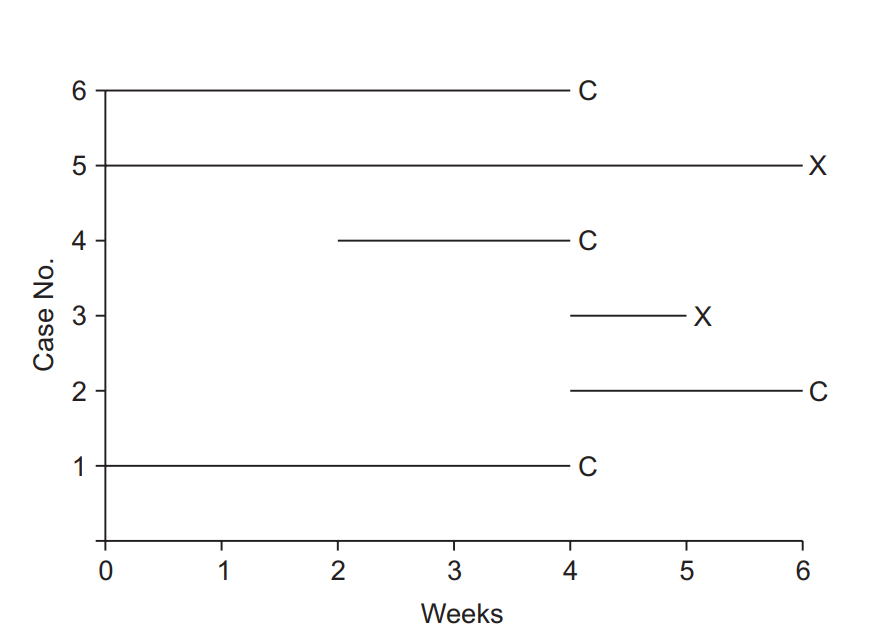
\includegraphics[width=1\linewidth]{Figure 3/3.2.png}
    \caption{Censoring Graph}
    \label{Figure 3.2}
\end{figure}



\vspace{0.1in}
 \noindent \(C\) indicates censored data
\\ \noindent  \(X\) indicates observed events






\section{Fundamental Concepts of Survival Analysis}

\subsection{\texorpdfstring{Survival Function \( S(t) \)}{Survival Function S(t)}}
The survival function \(S\left(t\right) \) also known as the survival probability function, gives the probability that a person survives longer than some specified time.  Let \(T\) be a non-negative continuous random variable representing the elapsed time until an event occurs. The probability density function (pdf) of \(T\) is denoted by \(f(t)\) and the cumulative distribution function (cdf) is denoted by \(F(t)\). The cdf \(F(t)\) is defined as:
\begin{equation}
F(t) = \Pr\{T < t\}
\end{equation}
The survival function \(S(t)\) is the complement of the cumulative distribution function and is given by:
\begin{equation}
S(t) = 1 - F(t)
\end{equation}
\begin{equation}
S(t) = \Pr\{T \geq t\}
\end{equation}
\begin{equation}
S(t) = \int_t^\infty f(u) \, du
\end{equation}
The derivative of \(S(t)\) with respect to \(t\) is:
\begin{equation}
S'(t) = -F'(t)
\end{equation}
\begin{equation}
S'(t) = -f(t)
\end{equation}
In Figure \ref{Figure 3.3} below, the curve on the left is a theoretical curve of the survival function\ \(S\left(t\right) \) which ranges from 0 up to infinity. It is non-increasing and therefore slopes downward as \(t\) increases. At \(t= 0\), \(S\left(0\right)=1\) and when \( t\ =\ \infty , S\left(\infty\right)\ =\ 0.\) When actual data is used, the survivor curve does not result in a smooth curve but rather obtains a step function graph. The step function is illustrated on the right in Figure \ref{Figure 3.3}.  The study period is never infinite in duration as there may be competing risks for failure, not everyone may obtain the event of interest. The estimated survivor function \(\hat{S}\left(t\right)\), thus may not go all the way down to 0 at the end of the study.

\begin{figure}[H]
    \centering
    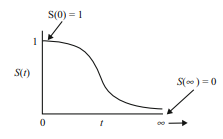
\includegraphics[width=0.45\textwidth]{Figure 3/3.31.png}
    \hfill
    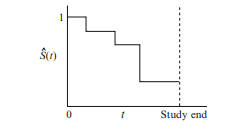
\includegraphics[width=0.45\textwidth]{Figure 3/3.32.png}
    \caption{Survivor Curves}
    \label{Figure 3.3}
\end{figure}



\subsection{\texorpdfstring{Hazard Function \( h(t) \)}{Hazard Function h(t)}}

The hazard function \( h(t)\ \)denotes the instantaneous rate of failure at time \(t\), given that the subject has survived up to time\( (t).\)

\begin{equation}
h(t) = \lim_{\Delta t \to 0} \frac{P(t \le T < t + \Delta t \mid T \geq t)}{\Delta t}
\end{equation}
\begin{equation}
h\left(t\right)\geq0
\end{equation}\\
The hazard function \( h\left(t\right)\), is given by the formula: \(h\left(t\right)\ \)equals the limit, as \(\Delta t \) approaches zero, of a probability statement about survival, divided by \(\Delta t\), where \(\Delta t\) denotes a small interval of time.

\begin{align}
h(t) &= \lim_{\Delta t \to 0} \frac{\Pr(t \leq T < t + \Delta t \mid T > t)}{\Delta t} \\
&= \lim_{\Delta t \to 0} \left[ \frac{\Pr(t \leq T < t + \Delta t)}{\Delta t} \cdot \frac{\Delta t}{\Pr(T > t)} \right] \\
&= \lim_{\Delta t \to 0} \left[ \frac{\Pr(t \leq T < t + \Delta t)}{\Delta t} \right] \cdot \lim_{\Delta t \to 0} \left[ \frac{1}{\Pr(T > t)} \right] \\
&= \frac{1}{S(t)} \cdot \lim_{\Delta t \to 0} \left[ \frac{\Pr(t \leq T < t + \Delta t)}{\Delta t} \right] \\
&= \frac{1}{S(t)} \cdot \lim_{\Delta t \to 0} \left[ \frac{F(t + \Delta t) - F(t)}{\Delta t} \right] \\
&= \frac{f(t)}{S(t)} 
\end{align}\\
The hazard function is also known as the conditional failure rate. It is a rate rather than a probability. In the hazard function formula, the expression to the right of the limit sign gives the ratio of two quantities. The numerator is a conditional probability while the denominator, \(\Delta t\) denotes a small-time interval. By the division, a probability per unit of time is obtained, which is no longer a probability but a rate. In particular, the scale for this ratio is not 0 to 1 like a probability but rather ranges between 0 and infinity while depending on whether time is measured in days, weeks, months, or years. 

\begin{equation}
H(t)=\int_{0}^{t}{h(x)dx}
\end{equation}\\
The cumulative hazard function \(H(t)\) can be derived from the hazard function. It is the integral of the hazard function up to time \(t\). It represents the total hazard experienced up to time \( t. H(t)\) provides a straightforward cumulative measure of risk or failure over time.

\begin{equation}
S(t) = \exp\left[-\int_{0}^{t} h(x) \, dx\right]
\label{eq:survival_function}
\end{equation}

\begin{equation}
h(t) = -\left[\frac{dS(t)/dt}{S(t)}\right]
\end{equation}\\
The equations above clearly defines the relation between the hazard function and survival function. This can be seen in (3.25) and (3.26) in which the $h(t)$ gives the $S(t)$ and vice versa.


\section{Approaches in Survival Analysis}

The approaches to use in survival analysis are underlined by their strengths and weaknesses. The choice is based on statistical assumptions, data characteristics and the complexity of the survival patterns to model.

\subsection{Parametric Methods}

Parametric survival analysis is based on the assumption that survival times conform to a particular statistical distribution. The exponential, weibull, log-normal, and gamma distributions are common models that can be applied to various kinds of survival data [Aalen, 2002]. Maximum likelihood estimation, which finds the values that best fit the observed data, is commonly used for parameter estimation. As an alternative, Bayesian techniques can be applied, which refine estimates based on data by combining previous knowledge.

\subsection{Non-Parametric Methods}

In survival analysis, non-parametric techniques are useful since they assume very little about the survival distribution. A popular tool for estimating survival probabilities and visualizing survival curves is the Kaplan-Meier Estimator. In contrast, the Nelson-Aalen Estimator calculates the cumulative hazard function and offers insights into the event's risk over time. The survival distributions of the groups are compared using the Log-Rank Test to see if there are any notable variations. When examining survival data and the precise distribution is unclear, these techniques can be helpful.




\subsection{Semi-Parametric Methods}

Semi-parametric models are used to assess survival data by combining parametric and non-parametric components. To accommodate different data patterns, they employ a non-parametric method to estimate the baseline hazard function and a parametric technique to represent the effect of variables. The Cox Proportional Hazards model is one illustration.

\section{Kaplan Meier}
The Kaplan-Meier estimator is employed in survival analysis to analyze the time until an event occurs. The Kaplan-Meier estimator calculates the survival probability at a specific time step by multiplying the probability of surviving each previous time step.
The estimator is computed as
\begin{equation}
S\left(t\right)=\prod_{i:t_i\le t}\left(1-\frac{d_i}{n_i}\right)
\end{equation}
Where:\\
     \(t\) is a time,\\
      \(d_i \) the number of events (churn) at time, \(t_i\)\\
      \(S\left(t\right)\ \)is the survival probability at time \(t\) and\\
      \(n_i\) is the number of individuals at risk just before time. \(t_i\)\\
\\ The estimator essentially calculates the probability of surviving from one time step to the next and the product of these probabilities gives the overall survival probability up to time \(t\).

\section{Cox Proportional (Cox PH) Hazard Model}

The Cox Proportional Hazards model is a popular semi-parametric model to check the relationship between the survival time and a set of predictors.

\begin{equation}
h\left(t \mid x\right) = h_0(t) \exp(\beta_1 x_1 + \beta_2 x_2 + \cdots + \beta_p x_p)
\end{equation}\\
Where:\\
\vspace{0.1in}
   \(h(t\mid x)\) is the hazard function, i.e., the instantaneous rate of the event occurring at time \(t\) given the predictor variables \(x\).\\
\vspace{0.1in}
   \(h_0\left(t\right)\) is the baseline hazard function, representing the hazard for individuals with all predictor variables equal to zero,\\
\vspace{0.1in}
     \(\beta_1,\beta_2,\ldots,\beta_p\) are the coefficients for the predictor variables.\\
\vspace{0.1in}
\\ The coefficients \(\beta\) are estimated using maximum likelihood estimation and the model assumes a proportional hazard ratio, meaning the effect of the predictors on the hazard is constant over time.
An important assumption on the Cox PH is that it has a constant hazard function proportion for each time. The Hypothesis of the assumption is as follows: 

$$H_0: \text{The Assumption of Proportional Hazard is fulfilled} $$
$$H_1: \text{The Assumption of Proportional Hazard is not fulfilled}$$
\\with the rejection test, if the $p-value < 0.05$, then the hazard ratios are constant over time.

\section{Accelerated Failure Time (AFT)}

When the Cox proportional hazards assumption is not satisfied, the parametric model approach can be used. Accelerated Failure Time (AFT) is one of the popular parametric models used in survival analysis. The model assumes that the survival function \(S(t)\) follows a parametric continuous distribution. This implies that the distribution follows a Weibull, lognormal, or log-logistic distribution. An AFT model aims to account for the influence of multiple covariates on the survival time by either accelerating or decelerating it.

\begin{equation}
\lambda(x) = \exp(b_0 + \sum_{i=1}^{n}{b_i x_i})
\end{equation}
Where:\\
\vspace{0.1in}
     \(\lambda(x)\) is the accelerating factor \\
\vspace{0.1in}
     \(b_0\) is the baseline accelerating factor when all covariates are 0 \\
\vspace{0.1in}
     \(b_i\) is the regression coefficient for the \(i\)-th covariate \\
\vspace{0.1in}
     \(x_i\) are the covariates\\




$$
H_0: \text{The covariates do not impact the survival time} $$
$$H_1: \text{The covariates have an impact on the survival time}$$\\
with the rejection test, if the $p-value < 0.05$, the covariates significantly affect the survival time in the AFT model.



\subsection{Weibull AFT}
Depending on its shape parameter, the Weibull distribution can model increasing, decreasing, or stable hazard rates, making it a very versatile tool in survival analysis. Because of its adaptability, it can be used for a variety of survival data, including medical outcomes and mechanical failures.

\begin{equation}
    S(t) = \exp\left(-\left(\frac{t}{\lambda}\right)^\gamma\right)
\end{equation}\\
where \(\lambda\) is the scale parameter and \(\gamma\) is the shape parameter.

\subsection{Lognormal AFT}
In the case of right-skewed data, the model assumes that the survival time has a normal distribution. It converts the survival time into a log-normal distribution, which fits skewed survival data better and can effectively depict data with a long right tail.

\begin{equation}
    S(t) = 1 - \Phi\left(\frac{\log(t) - \mu}{\sigma}\right)
\end{equation}\\
where \(\mu = b_0 + \sum_{i=1}^{n}{b_i x_i}\) is the location parameter, \(\sigma\) is the scale parameter and \(\Phi\) is the cumulative distribution function of the standard normal distribution.

\subsection{Log-logistic AFT}
The model can handle both growing and decreasing hazard rates, and it assumes that the survival time follows a logistic distribution. Like the Weibull model, it is adaptable and diverse, which makes it helpful for simulating various risk patterns across time.


\begin{equation}
    S(t) = \left(1 + \left(\frac{t}{\lambda}\right)^\gamma\right)^{-1}
\end{equation}\\
where \(\lambda\) is the scale parameter and \(\gamma\) is the shape parameter.


 
\section{Information Criteria and Loglikehood}

Information criteria are used to evaluate and compare the relative quality of statistical models. They help in model selection by balancing model fit with complexity and penalizing models that use more parameters to avoid overfitting.

\subsection{Log-Likelihood}

The log-likelihood function is used in measuring how well a model explains the observed data. It is the logarithm of the likelihood function, which represents the probability of observing the given data under a specific model.

\begin{equation}
\ln(L) = \sum_{i=1}^{n} \ln(f(y_i \mid \theta)),
\end{equation}\\
Where:\\
\vspace{0.1in}
     \(n\) is the number of observations. \\
\vspace{0.1in}
   \(y_i\) represents each data point. \\
\vspace{0.1in}
   \(f(y_i \mid \theta)\) is the probability density function of the data given the parameters \(\theta\). \\
\vspace{0.1in} \\
A higher log-likelihood value indicates that the model provides a better fit to the data. When comparing different models, the one with the highest log-likelihood is typically preferred, as it suggests that the model is more likely to have generated the observed data. However, it's important to balance this with model complexity, which is where information criteria like  Akaike Information Criterion (AIC), Bayesian Information Criterion (BIC) and Hannan-Quinn Criterion.

\subsection{Akaike Information Criterion (AIC)}

The Akaike Information Criterion (AIC) is a tool used to evaluate and compare statistical models. It balances the model's fit to the data with its complexity by penalizing models with more parameters. A lower AIC value indicates a better model, as it suggests a good fit with fewer parameters.

\begin{equation}
AIC = 2k - 2\ln(L),
\end{equation}\\
Where:\\
\vspace{0.1in}
     \(k\) is the number of parameters in the model. \\
\vspace{0.1in}
     \(L\) is the likelihood of the model. \\


\subsection{Bayesian Information Criterion (BIC)}
The Bayesian Information Criterion (BIC) is used for model selection, similar to AIC but with a stronger penalty for the number of parameters. This makes BIC more conservative, favoring simpler models, especially with larger sample sizes.

\begin{equation}
BIC = k\ln(n) - 2\ln(L),
\end{equation}\\
Where:\\
\vspace{0.1in}
     \(k\) is the number of parameters in the model.\\
\vspace{0.1in}
     \(n\) is the number of observations in the dataset.\\
\vspace{0.1in}
     \(L\) is the likelihood of the model.\\


\subsection{Hannan-Quinn Criterion (HQ)}
The Hannan-Quinn Criterion (HQ) is a model selection tool that lies between AIC and BIC in terms of penalizing model complexity. It provides an intermediate option, with a penalty for the number of parameters that is less severe than BIC but more stringent than AIC.

\begin{equation}
HQ = 2k\ln(\ln(n)) - 2\ln(L),
\end{equation}\\
Where:\\
\vspace{0.1in}
     \(k\) is the number of parameters in the model.\\
\vspace{0.1in}
     \(n\) is the number of observations in the dataset.\\
\vspace{0.1in}
     \(L\) is the likelihood of the model.



\section{Concordance Index in Survival Analysis}

A vital statistical metric used in survival analysis to evaluate the discriminative power of predictive models is the Concordance Index, also referred to as the C-index or Harrell's C-index [Harrell et al., 1982]. It is a gauge of a model's ability to distinguish across subjects with varying event durations, concentrating on the model's precision in assigning a person a risk rating.
In order to ascertain if people with higher expected risks actually experience events sooner than those with lower risks, the C-index assesses the concordance between the predicted risk scores and the actual event outcomes.

\begin{equation}
C=\frac{Number\ of\ Concordant\ Pairs}{Number\ of\ Concordant\ Pairs\ +Number\ of\ Discordant\ Pairs}
\end{equation}\\
This metric is particularly valuable in survival analysis because it provides a single, interpretable summary of the model's overall discriminatory power. A higher C-index indicates that the model is more accurate in predicting which subjects are at greater risk, making it an essential tool for evaluating and comparing the performance of different survival models. The C-index has become a standard measure in survival analysis and has been widely adopted in both clinical and research settings for validating the effectiveness of prognostic models.



\newpage
\chapter{Results and Analysis}
\section{Introduction}
This section presents the study's findings and discusses what each output means toward the research goals. It includes tables, graphs and computer results based on the methods used. The analysis closely examines details of the model building, diagnostics and evaluation. The information here was obtained from using python for computer analysis during the research. This chapter seeks to explain the use of survival models in the methodology to determine the Vodafone (Telecel) churn rate among students.


\section{Sample Size Calculation}
The sample size was calculated using the following parameters:
\vspace{0.3in}
\\
\vspace{0.1in}
{Z-score} \((z)\): A confidence level of 95\% is chosen, resulting in a Z-score of 1.96.\\
\vspace{0.1in}
{Population} \((N)\): The population size of the College of Science students is about 2,835.\\
\vspace{0.1in}
{Estimated Proportion} \((p)\): To maximize sample size, we use 0.5.\\
\vspace{0.1in}
{Margin of Error} \((E)\): 5\% since the confidence level is 95\%.\\


\begin{equation}
n_0 = \frac{\left(1.96^2 \times 0.5 \times 0.5\right)}{0.05^2}
\end{equation}
\begin{equation}
n_0 \approx 383.82
\end{equation}
\begin{equation}
n_0 \approx 384
\end{equation}
\begin{equation}
n = \frac{384}{1 + \left(\frac{384 - 1}{2835}\right)}
\end{equation}
\begin{equation}
n \approx 338.297
\end{equation}
\begin{equation}
n \approx 338
\end{equation}\\

\noindent From a population of 2,835 students in college of Science, a sample size of 338 students were selected.

\section{Data Description}

The dataset has a shape consisting of 338 rows and 14 columns from a sample of students in KNUST's College of Science. The Churn variable is assigned as the event while the Churn Level is assigned as the time to the event (duration). The remaining covariates are used to explain the event and duration.
\begin{table}[H]
    \centering
    \begin{tabularx}{\textwidth}{XXl}
        \toprule
        \textbf{Variable} & \textbf{Description} & \textbf{Data Type} \\
        \midrule
        Gender & The gender of the student & Categorical \\
        Churn & Whether the student has churned & Categorical \\
        Residence & Place of residence in school & Categorical \\
        Usage Frequency & Frequency of Vodafone Sim usage & Categorical \\
        Voice Calls & Usage of voice calls & Categorical \\
        Mobile Data Internet & Usage of mobile data/internet & Categorical \\
        SMS Text Messaging & Usage of SMS/text messaging & Categorical \\
        Data Exhaustion & Whether monthly data allowance (5GB) is exhausted & Categorical \\
        Multiple Networks & Use of other networks &Categorical \\
        Poor Network Quality Coverage & Perception of poor network quality/coverage & Categorical \\
        Unsatisfactory Customer Service & Perception of unsatisfactory customer service & Categorical \\
        High Costs Pricing & Perception of high costs/pricing & Categorical \\
        Monthly Data Usage & Monthly Data Usage & Categorical \\
        Churn Level & Level at which the student churns & Numeric \\
        \bottomrule
    \end{tabularx}
    \caption{Description of Variables}
    \label{tab: 4.1}
\end{table}
\noindent Table \ref{tab: 4.1} contains behavioral data like usage frequency, voice calls, and mobile data internet usage, in addition to demographic data like gender and place of residence.



\section{Descriptive Analysis}
\begin{figure}[H]
    \centering
    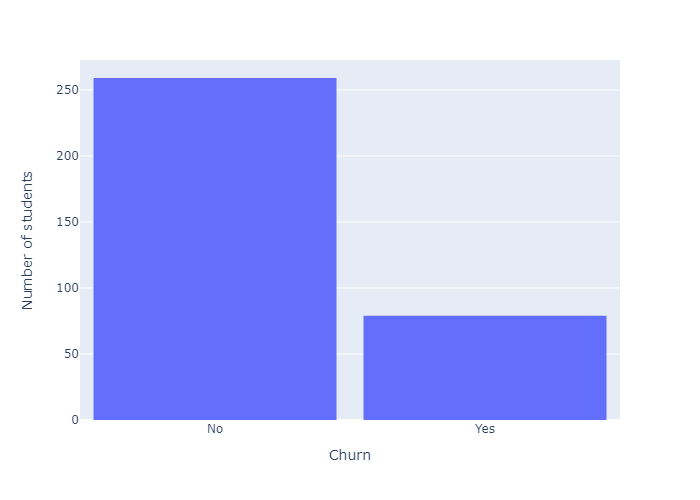
\includegraphics[width=1\linewidth, height=0.5\textheight]{Figure 4/distribution.png}
    \caption{Descriptive Analysis of Churn Data}
    \label{fig: Descriptive Analysis}
\end{figure}
In Figure \ref{fig: Descriptive Analysis} above, out of the 338 students, 79 were recorded to have churned. The survey also recorded 259 students who had not observed the event of interest (churn).

\begin{table}[H]
    \centering

    \begin{tabular}{llr}
        \toprule
        \textbf{Variable} & \textbf{Response} & \textbf{Number of students} \\
        \midrule
        \textbf{Gender} & Female & 233 \\
                        & Male & 105 \\
        \midrule
        \textbf{Churn} & No & 259 \\
                       & Yes & 79 \\
        \midrule
        \textbf{Residence} & Off-campus & 279 \\
                           & On-campus & 59 \\
        \midrule
        \textbf{Usage Frequency} & Daily & 170 \\
                                 & Several times a week & 67 \\
                                 & Occasionally & 60 \\
                                 & Never & 23 \\
                                 & Rarely & 18 \\
        \midrule
        \textbf{Voice Calls} & Yes & 285 \\
                             & No & 53 \\
        \midrule
        \textbf{Mobile Data Internet} & Yes & 302 \\
                                      & No & 36 \\
        \midrule
        \textbf{SMS Text Messaging} & Yes & 180 \\
                                     & No & 158 \\
        \midrule
        \textbf{Data Exhaustion} & Yes & 283 \\
                                  & No & 55 \\
        \midrule
        \textbf{Multiple Networks} & Yes & 312 \\
                                    & No & 26 \\
        \midrule
        \textbf{Poor Network Quality Coverage} & No & 276 \\
                                               & Yes & 62 \\
        \midrule
        \textbf{Unsatisfactory Customer Service} & Yes & 288 \\
                                                 & No & 50 \\
        \midrule
        \textbf{High Costs Pricing} & Yes & 291 \\
                                     & No & 47 \\
        \midrule
        \textbf{Monthly Data Usage} & 8 and more & 231 \\
                                    & 6-8 & 41 \\
                                    & 2-4 & 33 \\
                                    & 0-2 & 22 \\
                                    & 4-6 & 11 \\
        \bottomrule

    \end{tabular}
    \caption{Numbers of Responses for each Variable}
    \label{tab: description}
\end{table}
\noindent The response for the number of student in each variable is shown in Table \ref{tab: description}. The number of students who choose each response category is indicated next to it, giving a clear picture of the distribution of data across several variables.




\subsection{Kaplan Meier Analysis}

The provided Kaplan-Meier estimator output in Table 4.2 below summarizes the survival curve in Table 4.1 over the levels in KNUST.


\begin{table}[H]
\centering
\begin{tabularx}{\textwidth}{lXXXXX}
\toprule
Event Time & Number of Students & Churned Students & Survival Probability & Lower 95\% Confidence Interval & Upper 95\% Confidence Interval \\
\midrule
0 & 338 & 0 & 1.000000 & 1.000000 & 1.000000 \\
1 & 338 & 25 & 0.926036 & 0.892497 & 0.949406 \\
2 & 313 & 22 & 0.860947 & 0.819283 & 0.893630 \\
3 & 291 & 32 & 0.766272 & 0.717405 & 0.807836 \\ 
\bottomrule
\end{tabularx}
\caption{Kaplan-Meier Survival Analysis Results}
\label{tab:km_results}
\end{table}

\noindent Initially, at time 0 in Table \ref{tab:km_results} (when students initially start the academic year), all 338 students are considered to be at risk. With no events (churns) recorded yet, the survival probability is 1.\\
As the students ascend the academic ladder, the number at risk begins to gradually decrease as some begin to experience the event. The higher the number of events, the more the number at risk decreases. \\
At the end of the first year, 25 students experienced the event of interest and therefore were omitted from the study at the beginning of the second year. Anytime the event of interest is experienced, they are omitted from the study until the study duration ends.\\
The confidence intervals (Lower and Upper 95\% cond) provide ranges within which the true survival probabilities lie with a certain level of confidence.

\subsection{Kaplan Meier (KM) Curve}

The Kaplan-Meier survival curve below is a tool to estimate the probability that students will remain enrolled in the study over a given period. 
\begin{figure}[H]
    \centering
    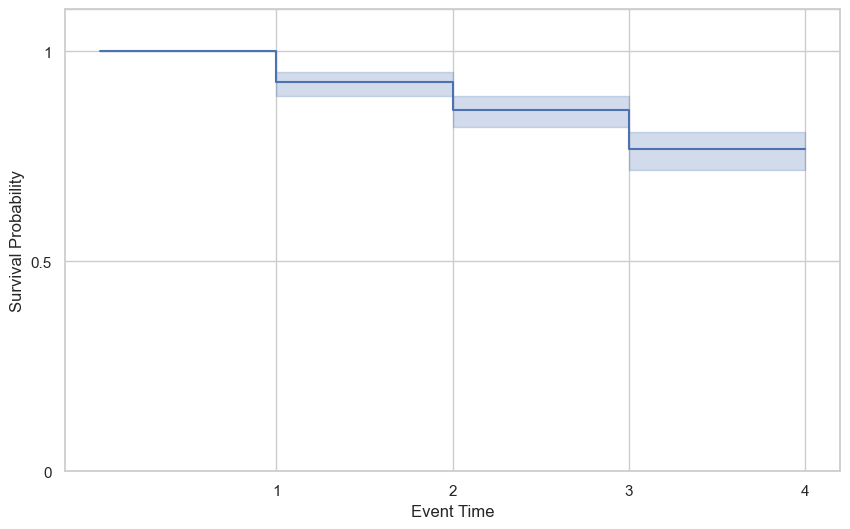
\includegraphics[width=1\linewidth]{Figure 4/4.1.png}
    \caption{Kaplan Meier Curve}
\end{figure}
\noindent  The x-axis represents the event time (Churn Level). The 0 indicates when the study began while the 4 represents when the study ended. The y-axis represents survival probability and ranges from 0 to 1. Each step down indicates an event, which decreases the overall survival probability.  The shaded area around the line suggests the confidence interval, giving a range within which the true survival curve is expected to lie.\\
In churn prediction, this curve helps identify critical time points where student retention drops significantly and allows institutions to intervene proactively. 



\section{Cox Proportional Hazard (COX PH)}

In the Cox Proportional Hazard modeling, two things are mostly done, namely, partial testing for each predictor variable and testing the Cox Proportional Hazard assumption.\\
Furthermore, the results of parameter estimation and partial testing are presented in the Table below.

% Insert another Table

\begin{table}[H]
\centering
\begin{tabular}{lccc}
\toprule
Variable & Coefficient ($\beta$) & Standard Error & P-value\\
\midrule
Gender & 0.33 & 0.28 & 0.24 \\
Residence & 0.32 & 0.27 & 0.25 \\
Usage Frequency & -0.08 & 0.07 & 0.27 \\
Voice Calls & -0.57 & 0.32 & 0.08 \\
Mobile Data Internet & 0.32 & 0.46 & 0.48 \\
SMS Text Messaging & 0.48 & 0.25 & 0.06 \\
Data Exhaustion & -0.20 & 0.38 & 0.61 \\
Multiple Networks & -0.13 & 0.44 & 0.78 \\
Poor Network Quality Coverage & 2.60 & 0.35 & $<$0.005*\\
Unsatisfactory Customer Service & -1.40 & 0.30 & $<$0.005*\\
High Costs Pricing & -1.13 & 0.29 & $<$0.005*\\
Monthly Data Usage & 0.21 & 0.09 & 0.02*\\
\bottomrule
\end{tabular}
\caption{Cox Proportional Hazards Model Results}
\label{tab:cox_ph_results}
\end{table}

{* indicates significant covariate.}
\vspace{0.4cm}\\
\normalsize{\noindent The coefficient columns in Table \ref{tab:cox_ph_results} provide information about the relationship between each independent variable and the dependent variable. A positive coefficient indicates an increase in the independent variable is associated with an increase in the hazard (risk) of churn (event). A higher value of these variables is associated with a higher likelihood of churn occurring. \\
Conversely, a negative coefficient suggests a decrease in the hazard (risk) of churn (event). A higher value of these variables is associated with a lower likelihood of churn occurring.\\
The p-value column helps assess the statistical significance of each independent variable. A low p-value ( \(<\) 0.05) indicates that the covariate is likely to have a meaningful impact on the event. This can be seen in Monthly Data Usage, Poor Network Quality Coverage and High Costs Pricing.

\begin{figure}[H]
    \centering
    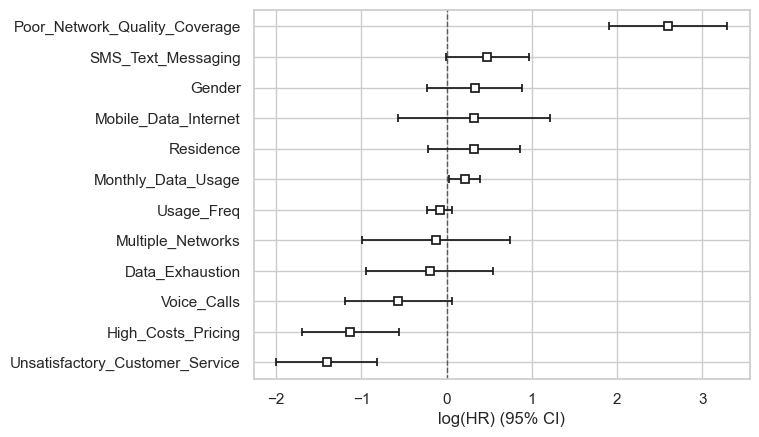
\includegraphics[width=1\linewidth]{Figure 4/4.2.png}
    \caption{Cox PH Forest Plot}
    \label{cox ph forest}
\end{figure}

\normalsize {\noindent Figure \ref{cox ph forest} above is a forest plot of the Cox PH. A coefficient to the right of zero (positive log hazard ratio) indicates that an increase in that variable is associated with a higher risk of a student churning. A coefficient to the left of zero (negative log hazard ratio) indicates that an increase in that covariate is associated with a lower risk of a student churning.
The further a coefficient is from zero, the stronger the effect of that covariate on the hazard of churn.
The horizontal lines extending from the boxes are the 95\% confidence intervals, showing the uncertainty around these estimates. If the confidence interval crosses zero, the covariate is not statistically significant.}

\subsection{Cox PH Assumption Test}
\normalsize{\noindent This test checks if the impact of the predictor variables on the hazard rate is constant over time. Covariates violating this assumption might need further investigation or transformation.\\	
The null hypothesis states that there is a significant relationship between the predictor variables (such as College and Voice Calls) and the likelihood of a student churning.\\
The alternative hypothesis suggests that there is no significant association between the predictor variables and the likelihood of churn.}

\begin{table}[H]
    \centering
    \begin{tabular}{lcc}
        \toprule
        Covariate & Test Statistic & P-value \\
        \midrule
        Data Exhaustion & 0.46 & 0.50 \\
        Gender & 0.26 & 0.61 \\
        High Costs Pricing & 1.74 & 0.19 \\
        Mobile Data Internet & 0.63 & 0.43 \\
        Monthly Data Usage & 1.49 & 0.22 \\
        Multiple Networks & 0.09 & 0.77 \\
        Poor Network Quality Coverage & 2.36 & 0.12 \\
        Residence & 0.01 & 0.93 \\
        SMS Text Messaging & 0.04 & 0.84 \\
        Unsatisfactory Customer Service & 0.10 & 0.76 \\
        Usage Frequency & 0.04 & 0.84 \\
        Voice Calls & 2.70 & 0.10 \\
        \bottomrule
    \end{tabular}
    \caption{Test statistics of Cox-PH Assumption Test}
    \label{tab:test_statistics}
\end{table}


\normalsize{\noindent The Cox Proportional Hazard method is an assumption that must be met. In Table \ref{tab:test_statistics}, it can be seen that the covariates meet the assumptions as their p-values are above 0.05 meaning that there is no strong evidence against the proportional hazard’s assumption for these covariates.\\
This means that the assumption that the hazard ratios are constant over time holds for all the covariates.}



\section{Accelerated Failure Time (AFT) }

\normalsize{The Accelerated Failure Time (AFT) model is a possible alternative that can be used when the Cox Proportional Hazard (PH) model does not hold. The study uses the AFT to understand the direct effect of covariates on survival time.}


\begin{table}[H]
    \centering
    \normalsize
    \begin{tabularx}{\textwidth}{lXXX}
        \toprule
        Model & AIC & BIC & Hanna-Quinn \\
        \midrule
        Weibull & 316.433303 & 300.079395 & 306.67379 \\
        \textbf{LogNormal} & \textbf{305.805320} & \textbf{289.451411} & \textbf{306.67379} \\
        LogLogistic & 307.510343 & 291.156435 & 306.67379 \\
        \bottomrule
    \end{tabularx}
    \caption{Comparison of AIC, BIC, and Hanna-Quinn values for different AFT models}
    \label{tab:model_comparison}
\end{table}



\noindent
\normalsize{\textbf{Results:} \\
The AFT model with the lowest AIC is: \textit{LogNormal} \\
The AFT model with the lowest BIC is: \textit{LogNormal} \\
The AFT model with the lowest Hanna-Quinn is: \textit{Weibull}

\noindent The study compares three Accelerated Failure Time (AFT) models—Weibull, Log-Normal and Log-Logistic—using AIC, BIC and Hanna-Quinn criteria in Table \ref{tab:model_comparison}. The results reveal that the Log-Normal  consistently has the lowest AIC and BIC, indicating a better overall fit despite the Weibull  achieving the lowest Hanna-Quinn value.}

\subsection{Log-Normal Model}
% Table here


\begin{table}[H]
\centering
\begin{tabular}{lccc}
\toprule
Variable & Coefficient (${\beta}$)& Standard Error (SE) & P-value\\
\midrule
Data Exhaustion& 0.102 & 0.148 & 0.493 \\
Gender & 0.032 & 0.118 & 0.785 \\
High Costs Pricing & 0.515 & 0.122 & $<$0.0005*\\
Mobile Data Internet & -0.287 & 0.207 & 0.165 \\
Monthly Data Usage & -0.069 & 0.044 & 0.113 \\
Multiple Networks & -0.104 & 0.202 & 0.607 \\
Poor Network Quality Coverage & -1.041 & 0.123 & $<$0.0005*\\
Residence & -0.146 & 0.124 & 0.239 \\
SMS Text Messaging & -0.228 & 0.108 & 0.036*\\
Unsatisfactory Customer Service & 0.809 & 0.122 & $<$0.0005*\\
Usage Frequency & -0.002 & 0.033 & 0.940 \\
Voice Calls & 0.132 & 0.135 & 0.329 \\
Intercept (for $\mu$) & 1.626 & 0.393 & $<$0.0005\\
Intercept (for $\sigma$) & -0.616 & 0.084 & $<$0.0005\\
\bottomrule
\end{tabular}
\caption{Lognormal Model Coefficients}
\label{table:lognormal_coefficients}
\end{table}
{* indicates significant covariate.}
\vspace{0.4cm}\\
\normalsize{\noindent Unlike the Cox PH analysis, the coefficient columns in Table \ref{table:lognormal_coefficients} provide information about the relationship between the covariates to event time (Churn\_Level). A positive coefficient indicates a decrease in the time it takes to the event. A negative coefficient suggests an increase in the time to the event. }

\normalsize{\noindent A higher value of these covariates is associated with a higher  likelihood of the time to the event occurring if positive and a lower chance of occurring if negative.}
 
\normalsize{\noindent The p-value column helps assess the statistical significance of each covariate. A low p-value ( \(< \) 0.05) indicates that the covariate is likely to have a meaningful impact on Churn Level. }

\normalsize{\noindent The mu\_intercept is the mean baseline when the covariates are 0 and the sigma\_intercept is the standard deviation used to estimate the variance to determine the spread when the covariates are 0.}

\begin{figure}[H]
    \centering
    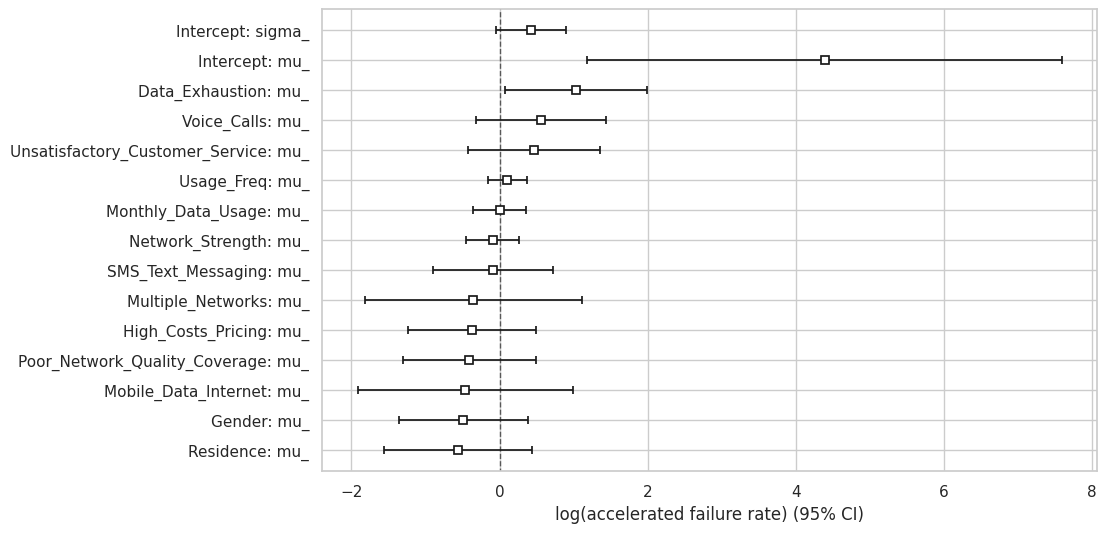
\includegraphics[width=1\linewidth]{Figure 4/4.4.png}
    \caption{LogNormal Forest Plot}
    \label{LogNormal}
\end{figure}

\normalsize{\noindent The boxes (squares) in the plot represent the estimated coefficients for each factor in the Lognormal AFT model in Figure \ref{LogNormal}. The positive values suggest that the covariate decreases the time to the event (churn), while negative values suggest it increases the time to the event (Churn Level). The horizontal lines extending from the boxes are the 95\% confidence intervals, showing the uncertainty around these estimates. If the confidence interval crosses zero, the covariate is not statistically significant.}

\section{Model Comparison}

\normalsize{\noindent In this section, the models used are compared based on the Loglikelihood and the concordance values. The higher the concordance, the better the model predictive value and the higher the loglikelihood, the better the model fit.}

%Table here
	\begin{table}[H]
			\centering
			\begin{tabular}{lcc}
				\toprule
				\textbf{Model} & \textbf{Concordance} & \textbf{Loglike hood}\\
				\midrule
				LogNormal& 0.958& 	290.678\\
				Cox PH & 0.96& 	266.68\\
				\bottomrule
			\end{tabular}
			\caption{Model Concordance and AIC values}
			\label{Table 2}
			
		\end{table}

\normalsize{\noindent Based on the comparison of the concordance values and log-likelihood in Table \ref{Table 2}, it is evident that the Cox PH model shows a higher concordance compared to the LogNormal model, indicating a better predictive value. However, the log-likelihood values suggest that the LogNormal model has a better fit. }

\newpage
\chapter{Summary of findings, conclusion and recommendations}

\section{Introduction}
\normalsize{ This section provides a comprehensive overview of the findings, conclusions, and recommendations derived from the study. The primary objective of the research was to investigate student churn of Telecel in KNUST, aiming to provide actionable insights and guidance based on the data analyzed.}

\section{Summary of finding}
Poor network quality, poor customer service, high costs pricing, monthly data usage, and SMS text messaging were found to be important indicators of student churn. While the Lognormal Accelerated Failure Time (AFT) model provided a higher and better log-likelihood value, the Cox Proportional Hazards (PH) model showed a higher and better concordance value. Furthermore, students churned more at the end of their 3rd year.

\section{Conclusion}
\normalsize{The analysis identified that out of the significant covariates—Poor network quality, poor customer service, high costs pricing, monthly data usage, and SMS text messaging —Poor Network Quality Coverage was the most significant covariate to increase both the churn rate and time to churn. The Cox Proportional Hazards model showed a higher predictive value, while the Lognormal Accelerated Failure Time (AFT) model provided a better fit for the data. Additionally, students in their 3rd year had the highest churn rate, with 35 out of 79 churners coming from this group.}

 



\section{Recommendations}
\normalsize{This section presents recommendations based on the study’s findings. From the analysis of the level 400 students in the College of Science over the 4 years, recommendations to the University Information Technology Services (UITS)  are as follows:}
\begin{enumerate}
        \item \normalsize{Improving network coverage at KNUST can reduce churn rates by ensuring consistent and reliable connectivity. This enhances students' access to online resources, supports smooth communication and minimizes technical issues, leading to a better overall academic experience and higher student satisfaction. Investing in better infrastructure and regular maintenance will help achieve these improvements}.

    \item  \normalsize{Establishing diverse communication channels and feedback systems through digital platforms ensures that students can get timely and efficient help. This 	approach addresses concerns effectively and improves overall student satisfaction.}
 
	\item \normalsize{Future research could expand on this study by including other Colleges in KNUST to obtain a more diverse student population. Using data from the UITS will capture student sentiments more deeply in understanding the churn of Telecel.}

\end{enumerate}









\chapter*{References}
\addcontentsline{toc}{chapter}{References}


\begin{enumerate}[label=\textbf{[\arabic*]}]


\item Bandim, M. (2022). Growth of Ghana's telecommunications industry. \textit{Journal of African Telecommunications}, 45(2), 123-135.

\item Ghana Web. (2024). Underwater fiber optic cable outages impact telecommunications in West Africa. \textit{Retrieved from:} \url{https://www.ghanaweb.com/GhanaHomePage/business/Details-of-the-outages-on-multiple-submarine-optic-fibre-cables-that-hit-MTN-Ghana-others-1921650}. Accessed: 2024-06-05.

\item Kapur, R. (2018). Factors driving customer churn in telecom industry. \textit{International Journal of Telecom Studies}, 22(4), 321-334.

\item Koranchirath, A. (2024). Customer retention strategies in competitive markets. \textit{Telecom Review}, 30(1), 56-72.

\item Masarifoglu, M., \& Buyuklu, A. H. (2019). Applying survival analysis to telecom churn data. \textit{American Journal of Theoretical and Applied Statistics}, 8(6), 261-275.

\item Nurhaliza, S., Sadik, K., \& Saefuddin, A. (2022). A comparison of Cox proportional hazard and random survival forest models in predicting churn of the telecommunication industry customer. \textit{BAREKENG: Jurnal Ilmu Matematika dan Terapan}, 16(4), 1433-1440.

\item Graunt, J. (1977). Natural and political observations mentioned in a following index, and made upon the bills of mortality. \textit{Mathematical Demography}, 6, 11-20.

\item Imani, M. (2020). Customer churn prediction in telecommunication using machine learning: A comparison study. \textit{AUT Journal of Modeling and Simulation}, 52(2), 229-250.

\item AP News. (2024). Underwater cable disruptions affect West Africa's internet services. \textit{Retrieved from:} \url{https://apnews.com/article/africa-internet-outage-undersea-cables-failure-ac67fd11b4d9ae7cb3959622c5e9e78b}. Accessed: 2024-06-05.

\item Alqatani, A., \& Altarifi, A. (2020). Title of the paper. \textit{Journal Name}, Volume(Issue), Pages.

\item Box-Steffensmeier, J., \& Jone, C. (2020). Title of the paper. \textit{Journal Name}, Volume(Issue), Pages.

\item Lai, T., et al. (2021). Title of the paper. \textit{Journal Name}, Volume(Issue), Pages.

\item Smith, R., \& Brown, J. (2020). Title of the paper. \textit{Journal Name}, Volume(Issue), Pages.

\item Jerenz, A. (2008). Title of the paper. \textit{Journal Name}, Volume(Issue), Pages.

\item Kaplan, E., \& Meier, P. (1958). Title of the paper. \textit{Journal Name}, Volume(Issue), Pages.

\item Cox, D. (1972). Title of the paper. \textit{Journal Name}, Volume(Issue), Pages.

\item Lee, M. (2014). Business bankruptcy prediction based on survival analysis approach. \textit{International Journal of Computer Science Information Technology}, 6(2), Pages.

\item Pereira, J. (2014). Survival analysis employed in predicting corporate failure: A forecasting model proposal. \textit{International Business Research}, 7(6), Pages.

\item Kumar, K., \& Gepp, A. (2015). Predicting financial distress: A comparison of survival analysis and decision tree techniques. \textit{Procedia Computer Science}, 54(2), 396-404.

\item Iwasaki, I. (2014). Global financial crisis, corporate governance, and firm survival: The Russian experience. \textit{Journal of Comparative Economics}, 42(1), 178-211.

\item Leung, M.K., Rigby, D., \& Young, T. (2010). Entry of foreign banks in the People's Republic of China: A survival analysis. \textit{Journal of Applied Economics}, 10, 21-31.

\item Evrensel, A.Y. (2008). Banking crisis and financial structure: A survival-time analysis. \textit{International Review of Economics and Finance}, 17(4), 589-602.

\item Tsujitani, M., \& Baesens, B. (2012). Survival analysis for personal loan data using generalized additive models. \textit{Behaviormetrika}, 39(1), 9-23.

\item Baesens, B., Gestel, T.V., Stepanova, M., Poel, D.V., \& Vanthienen, J. (2005). Neural network survival analysis for personal loan data. \textit{Journal of the Operational Research Society}, 56(9), 1089-109.

\item Cox, D.R., \& Lewis, P.A.W. (1972). Multivariate point processes. In \textit{Proceedings of the Sixth Berkeley Symposium on Mathematical Statistics and Probability}, Vol. 3, pp. 401-448.

\item Harrell, F.E., Califf, R.M., Pryor, D.B., Lee, K.L., \& Rosati, R.A. (1982). Evaluating the yield of medical tests. \textit{JAMA}, 247(18), 2543-2546.

\item Aalen, O.O. (2002). 1. The statistical analysis of failure time data (2nd edn). \textit{Prentice LR, Wiley-Interscience, Hoboken, New Jersey.}

\item Wikipedia. (2020). Vodafone Ghana. \textit{Retrieved from:} \url{https://en.wikipedia.org/wiki/Vodafone_Ghana#:~:text=As%20of%20January%202020%2C%20it,of%20the%20Ghanaian%20market%20shares}. Accessed: 2024-05-24.

\item Wikipedia. (2020). Vodafone KNUST. \textit{Retrieved from:} \url{https://en.m.wikipedia.org/wiki/Vodafone_Ghana#:~:text=In%202016%2C%20Vodafone%20made%20a,the%20university's%20campuses%20in%20Ghana}. Accessed: 2024-07-02.

\item Wikipedia. (2024). Telecel Ghana. \textit{Retrieved from:} \url{https://en.m.wikipedia.org/wiki/Telecel_Ghana#:~:text=They%20are%20the%20leading%20total,Vodafone%20Ghana%20into%20Telecel%20Ghana}. Accessed: 2024-05-19.

\end{enumerate}



\end{document}
 